Bij een live applicatie is het belangrijk dat de aangesloten apparaten de mogelijkheid hebben synchroon een beeld weer te geven. Dit is niet altijd vanzelfsprekend dankzij verschillende factoren, zoals vertraging op en snelheid van een apparaat. Hiervoor zijn er verschillende technieken om toch synchronisatie te bekomen.

\subsection{Vertraging berekenen}
Er is een vertraging tussen een aangesloten client en de server, de {\it ping}. Dit is gemeten in miliseconden.
Deze wordt gemeten door een bericht met de actuele tijd te verzenden van de server naar de client, en terug. De verzonden tijd wordt afgetrokken van de actuele tijd waarmee de ping verkregen is.
In figuur \ref{diag} is de informatieoverdracht zichtbaar. In de server wordt de servertijd (TS1) berekent, verzonden naar de client en teruggekregen.
Nu wordt de actuele tijd berekent in de server TS2. Dus de uiteindelijke ping is:
\[ping = TS2 - TS1\]

\tikzstyle{client} = [rectangle, rounded corners, minimum width=3cm, minimum height=2cm,text centered, draw=black, fill=blue!30]


\begin{figure}
    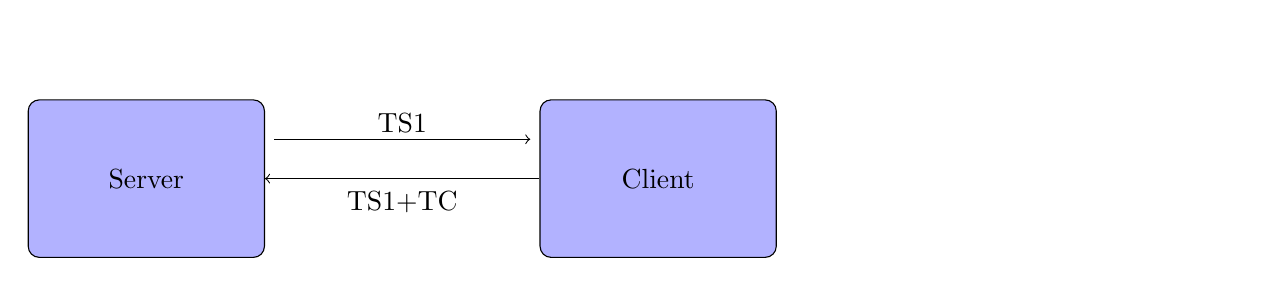
\begin{tikzpicture}[node distance=1.5cm and 2cm]

        \node (A) at (3.5, 1.5){};
        \node (B) at (8,1.5){};
        \node (C) at (6,1.8){};
        \node[red] (D) at (10,0.4){};
        \node (S1) at (1.5cm,0.5cm){};
        \node (S1T) at (3.25cm, 0.7cm){TS1};
        \node (C2T) at (3.25cm, -0.3cm){TS1+TC};
        \node (C1) at (5cm,0.5cm){};
        \node (F) at (12,1.5){};
        \node (G) at (14,1.5){};
        \node (H) at (13,1.7){};

        \node (serv) [client] {Server};
        \node (clie) [client, right of=serv, xshift=5cm] {Client};

        \path[->]
        (S1) edge  (C1)
        (clie) edge (serv);

    \end{tikzpicture}
    \caption{Diagram van informatieoverdracht. (TS: Time Server, TC: Time Client)} \label{diag}
\end{figure}

\begin{figure}
    \begin{lstlisting}[language=json,firstnumber=1]
    {
    type: 'count-down',
    data: {
    start: [integer]
    interval: [integer, in ms],
    startTime: [date in ms]
    }
    }
    \end{lstlisting}
    \caption{countdown JSON commando verzonden naar clients} \label{json2}
\end{figure}

\subsection{Kloksynchronisatie}
Het is niet gegarandeerd dat de klokken van de clients allemaal gesynchroniseerd zijn met de server. Daarom is het ook nodig om te weten wat het verschil is tussen de tijd aan de kant van de client en de server.
Bij het terug verzenden van de client naar de server wordt de clienttijd (TC) bij het bericht gezet. Met deze TC en de berekende {\it ping}, is het mogelijk het tijdsverschil tussen de client en de server te bepalen ($DeltaTime$). Door dit verschil toe te voegen aan de servertijd is het mogelijk de correcte clienttijd te vinden. Dit wordt gebruikt om een starttijd te bepalen voor elke client dat op exact hetzelfde moment zal beginnen:
\[DeltaTime = (TC+ping/2) - TS2\]

Zo is de tijd van de client ten opzichte van de server altijd:
\[TimeClient = TimeServer + DeltaTime\]


\subsection{Aftelklok}
Bij de naïeve implementatie van de aftelklok is er gebruik gemaakt van de {\it setTimer()}-functie die recursief een getal aftelt en tekent op een canvas. Een probleem hierbij is dat apparaten niet even snel het getal kunnen tekenen op het scherm waardoor er apparaten kunnen zijn die sneller zijn dan anderen.
Daarom is er gebruik gemaakt van {\it setInterval()} dat periodisch het getal berekent, relatief ten opzichte van de meegegeven starttijd. Als er een client trager is en niet op tijd op het scherm kan tekenen, dan zal het getal worden overgeslagen omdat het apparaat het sowieso niet zou aankunnen. Hierdoor blijven de getallen op het scherm synchroon en zal het aftellen ook op hetzelfde moment stoppen op elk scherm.
Het getal is als volgt berekend:
\[number = startNum - Math.floor((actualTime - startTime) / interval)\]


